% Options for packages loaded elsewhere
\PassOptionsToPackage{unicode}{hyperref}
\PassOptionsToPackage{hyphens}{url}
\PassOptionsToPackage{dvipsnames,svgnames,x11names}{xcolor}
%
\documentclass[
  a4paper,
]{article}

\usepackage{amsmath,amssymb}
\usepackage{iftex}
\ifPDFTeX
  \usepackage[T1]{fontenc}
  \usepackage[utf8]{inputenc}
  \usepackage{textcomp} % provide euro and other symbols
\else % if luatex or xetex
  \usepackage{unicode-math}
  \defaultfontfeatures{Scale=MatchLowercase}
  \defaultfontfeatures[\rmfamily]{Ligatures=TeX,Scale=1}
\fi
\usepackage{lmodern}
\ifPDFTeX\else  
    % xetex/luatex font selection
\fi
% Use upquote if available, for straight quotes in verbatim environments
\IfFileExists{upquote.sty}{\usepackage{upquote}}{}
\IfFileExists{microtype.sty}{% use microtype if available
  \usepackage[]{microtype}
  \UseMicrotypeSet[protrusion]{basicmath} % disable protrusion for tt fonts
}{}
\makeatletter
\@ifundefined{KOMAClassName}{% if non-KOMA class
  \IfFileExists{parskip.sty}{%
    \usepackage{parskip}
  }{% else
    \setlength{\parindent}{0pt}
    \setlength{\parskip}{6pt plus 2pt minus 1pt}}
}{% if KOMA class
  \KOMAoptions{parskip=half}}
\makeatother
\usepackage{xcolor}
\usepackage[top=2.54cm,right=2.54cm,bottom=2.54cm,left=2.54cm]{geometry}
\setlength{\emergencystretch}{3em} % prevent overfull lines
\setcounter{secnumdepth}{-\maxdimen} % remove section numbering
% Make \paragraph and \subparagraph free-standing
\ifx\paragraph\undefined\else
  \let\oldparagraph\paragraph
  \renewcommand{\paragraph}[1]{\oldparagraph{#1}\mbox{}}
\fi
\ifx\subparagraph\undefined\else
  \let\oldsubparagraph\subparagraph
  \renewcommand{\subparagraph}[1]{\oldsubparagraph{#1}\mbox{}}
\fi


\providecommand{\tightlist}{%
  \setlength{\itemsep}{0pt}\setlength{\parskip}{0pt}}\usepackage{longtable,booktabs,array}
\usepackage{calc} % for calculating minipage widths
% Correct order of tables after \paragraph or \subparagraph
\usepackage{etoolbox}
\makeatletter
\patchcmd\longtable{\par}{\if@noskipsec\mbox{}\fi\par}{}{}
\makeatother
% Allow footnotes in longtable head/foot
\IfFileExists{footnotehyper.sty}{\usepackage{footnotehyper}}{\usepackage{footnote}}
\makesavenoteenv{longtable}
\usepackage{graphicx}
\makeatletter
\def\maxwidth{\ifdim\Gin@nat@width>\linewidth\linewidth\else\Gin@nat@width\fi}
\def\maxheight{\ifdim\Gin@nat@height>\textheight\textheight\else\Gin@nat@height\fi}
\makeatother
% Scale images if necessary, so that they will not overflow the page
% margins by default, and it is still possible to overwrite the defaults
% using explicit options in \includegraphics[width, height, ...]{}
\setkeys{Gin}{width=\maxwidth,height=\maxheight,keepaspectratio}
% Set default figure placement to htbp
\makeatletter
\def\fps@figure{htbp}
\makeatother

\makeatletter
\makeatother
\makeatletter
\makeatother
\makeatletter
\@ifpackageloaded{caption}{}{\usepackage{caption}}
\AtBeginDocument{%
\ifdefined\contentsname
  \renewcommand*\contentsname{Tabla de contenidos}
\else
  \newcommand\contentsname{Tabla de contenidos}
\fi
\ifdefined\listfigurename
  \renewcommand*\listfigurename{Listado de Figuras}
\else
  \newcommand\listfigurename{Listado de Figuras}
\fi
\ifdefined\listtablename
  \renewcommand*\listtablename{Listado de Tablas}
\else
  \newcommand\listtablename{Listado de Tablas}
\fi
\ifdefined\figurename
  \renewcommand*\figurename{Figura}
\else
  \newcommand\figurename{Figura}
\fi
\ifdefined\tablename
  \renewcommand*\tablename{Tabla}
\else
  \newcommand\tablename{Tabla}
\fi
}
\@ifpackageloaded{float}{}{\usepackage{float}}
\floatstyle{ruled}
\@ifundefined{c@chapter}{\newfloat{codelisting}{h}{lop}}{\newfloat{codelisting}{h}{lop}[chapter]}
\floatname{codelisting}{Listado}
\newcommand*\listoflistings{\listof{codelisting}{Listado de Listados}}
\makeatother
\makeatletter
\@ifpackageloaded{caption}{}{\usepackage{caption}}
\@ifpackageloaded{subcaption}{}{\usepackage{subcaption}}
\makeatother
\makeatletter
\@ifpackageloaded{tcolorbox}{}{\usepackage[skins,breakable]{tcolorbox}}
\makeatother
\makeatletter
\@ifundefined{shadecolor}{\definecolor{shadecolor}{rgb}{.97, .97, .97}}
\makeatother
\makeatletter
\makeatother
\makeatletter
\makeatother
\ifLuaTeX
\usepackage[bidi=basic]{babel}
\else
\usepackage[bidi=default]{babel}
\fi
\babelprovide[main,import]{spanish}
% get rid of language-specific shorthands (see #6817):
\let\LanguageShortHands\languageshorthands
\def\languageshorthands#1{}
\ifLuaTeX
  \usepackage{selnolig}  % disable illegal ligatures
\fi
\usepackage[]{biblatex}
\addbibresource{../../../../references.bib}
\IfFileExists{bookmark.sty}{\usepackage{bookmark}}{\usepackage{hyperref}}
\IfFileExists{xurl.sty}{\usepackage{xurl}}{} % add URL line breaks if available
\urlstyle{same} % disable monospaced font for URLs
\hypersetup{
  pdftitle={Perspectivas Monetarias Globales. Análisis de Regímenes Cambiarios y el Futuro del FMI},
  pdfauthor={Edison Achalma},
  pdflang={es},
  colorlinks=true,
  linkcolor={blue},
  filecolor={Maroon},
  citecolor={Blue},
  urlcolor={Blue},
  pdfcreator={LaTeX via pandoc}}

\title{Perspectivas Monetarias Globales. Análisis de Regímenes
Cambiarios y el Futuro del FMI}
\usepackage{etoolbox}
\makeatletter
\providecommand{\subtitle}[1]{% add subtitle to \maketitle
  \apptocmd{\@title}{\par {\large #1 \par}}{}{}
}
\makeatother
\subtitle{Explorando los sistemas monetarios internacionales, tipos de
cambio fijos y flexibles, y el papel en evolución del FMI en la economía
mundial.}
\author{Edison Achalma}
\date{2023-06-17}

\begin{document}
\maketitle
\ifdefined\Shaded\renewenvironment{Shaded}{\begin{tcolorbox}[enhanced, interior hidden, breakable, borderline west={3pt}{0pt}{shadecolor}, boxrule=0pt, frame hidden, sharp corners]}{\end{tcolorbox}}\fi

\hypertarget{el-sistema-monetario-internacional}{%
\section{El Sistema Monetario
Internacional}\label{el-sistema-monetario-internacional}}

El sistema monetario internacional es un marco institucional establecido
para facilitar los pagos internacionales, regular los flujos de capital
y determinar los tipos de cambio entre las diferentes monedas. Este
sistema se basa en acuerdos internacionales y requiere un alto grado de
cooperación entre los gobiernos de los principales países. En el
contexto de la globalización, donde los flujos internacionales de
bienes, servicios y capitales son cada vez más intensos, se hace
necesaria la existencia de instituciones que regulen y faciliten estas
transacciones.

\hypertarget{reguxedmenes-cambiarios-y-apertura}{%
\subsection{Regímenes cambiarios y
apertura}\label{reguxedmenes-cambiarios-y-apertura}}

Es importante destacar que los países pueden seguir diferentes reglas en
lo que respecta a los regímenes cambiarios y el grado de apertura de sus
economías. Algunos países optan por tipos de cambio fijos, donde el
valor de su moneda se mantiene constante en relación con otra moneda o
una canasta de monedas. Otros países tienen tipos de cambio flexibles,
donde el valor de su moneda fluctúa en respuesta a las fuerzas del
mercado. Además, el grado de apertura de una economía se refiere a la
medida en que permite el comercio internacional y los flujos de capital.

\hypertarget{volatilidad-y-tipos-de-cambio}{%
\subsection{Volatilidad y tipos de
cambio}\label{volatilidad-y-tipos-de-cambio}}

En la actualidad, los mercados financieros internacionales se
caracterizan por una alta volatilidad en todas las variables económicas,
especialmente en los tipos de cambio. Esta volatilidad se debe a las
constantes modificaciones de las variables económicas, el progreso
tecnológico y la liberalización financiera. Los tipos de cambio fluctúan
en respuesta a factores como las tasas de interés, la inflación, los
flujos de capital y los eventos económicos y políticos a nivel mundial.

\hypertarget{divisas-y-cotizaciuxf3n-de-tipos-de-cambio}{%
\subsection{Divisas y cotización de tipos de
cambio}\label{divisas-y-cotizaciuxf3n-de-tipos-de-cambio}}

Una divisa es la moneda de otro país, siempre y cuando sea libremente
convertible a otras monedas en el mercado cambiario. La cotización del
tipo de cambio se refiere a la forma en que se establece el valor de una
moneda en relación con otra. La manera más común de cotizar el tipo de
cambio es mediante la cantidad de la moneda nacional necesaria para
comprar un dólar estadounidense (USD). Por ejemplo, si se requieren 1.5
unidades de la moneda nacional para comprar 1 USD, se diría que el tipo
de cambio es de 1.5.

\hypertarget{reguxedmenes-cambiarios}{%
\section{Regímenes Cambiarios}\label{reguxedmenes-cambiarios}}

El régimen cambiario se refiere a un conjunto de reglas que describen el
papel que desempeña el Banco Central en la determinación del tipo de
cambio. El Fondo Monetario Internacional (FMI) clasifica los regímenes
cambiarios en ocho categorías, que van desde aquellos donde no existe
una moneda nacional legal hasta aquellos basados en la flotación libre
del tipo de cambio. Cada régimen tiene implicaciones diferentes para la
política monetaria, la estabilidad económica y el comercio
internacional.

\textbf{1. No existe moneda nacional legal}

En este régimen, el país no tiene su propia moneda nacional legal y
utiliza la moneda de otro país, como el dólar estadounidense o el euro,
como medio de pago y unidad de cuenta. Ejemplos de países en este
régimen son Ecuador y Panamá, que adoptaron el dólar estadounidense como
su moneda oficial.

\textbf{2. Consejo monetario o Caja de conversión}

Este régimen se basa en un compromiso legislativo en el que se establece
que la moneda nacional debe cambiarse por una moneda extranjera
específica a un tipo de cambio determinado. Las autoridades emisoras
aceptan restricciones para cumplir con esta obligación legal. Ejemplos
de países con este régimen son Bosnia y Herzegovina, Brunei, Bulgaria,
Hong Kong, Djibouti y Estonia.

\textbf{3. Moneda nacional pegada a una moneda o una canasta de monedas}

En este régimen de tipo de cambio fijo o convertible, el país vincula su
moneda a una moneda importante o a una canasta de monedas. El valor del
tipo de cambio se determina en función del valor de las monedas de los
principales socios comerciales o financieros. Dentro de este régimen,
existe el régimen de tipo de cambio fijo, donde el tipo de cambio
fluctúa dentro de un margen estrecho alrededor de un tipo central
establecido.

\textbf{4. Moneda nacional pegada, pero dentro de bandas horizontales}

En este régimen, la moneda nacional se mantiene dentro de ciertos
márgenes de fluctuación en torno a un tipo de cambio central fijo.
Algunos países también participan en el mecanismo de tipos de cambio del
sistema monetario europeo. La amplitud de la banda determina el grado de
discrecionalidad de la política monetaria. Ejemplos de países en este
régimen son Dinamarca, Chipre, Egipto, Hungría y Tonga.

\textbf{5. Tipo de cambio de ajuste gradual}

En este régimen, el tipo de cambio se ajusta periódicamente en pequeñas
magnitudes, ya sea a una tasa fija o en respuesta a cambios en
indicadores cuantitativos. El objetivo es generar ajustes en el valor de
la moneda en línea con la inflación retrospectiva o proyectada. Se
imponen restricciones a la política monetaria para mantener el tipo de
cambio flexible, similar a un régimen de tipo de cambio fijo. Ejemplos
de países en este régimen son Bolivia, Costa Rica, Nicaragua e Islas
Salomón.

\textbf{6. Tipo de cambio ajustable dentro de una banda}

En este régimen, la moneda se mantiene dentro de ciertos márgenes de
fluctuación alrededor de un tipo de cambio central, que se ajusta
periódicamente a una tasa fija o en respuesta a cambios en indicadores
cuantitativos. El grado de flexibilidad del tipo de cambio depende de la
amplitud de la banda. Puede haber bandas simétricas alrededor de un tipo
central móvil o bandas asimétricas que se amplían gradualmente. La
política monetaria está limitada por la necesidad de mantener el tipo de
cambio dentro de la banda.

\textbf{7. Flotación administrada sin una ruta anunciada}

En este régimen, la autoridad monetaria interviene activamente en el
mercado cambiario para determinar el tipo de cambio, sin comprometerse
con una trayectoria preanunciada. Se utilizan indicadores como el saldo
de la Balanza de Pagos, las reservas internacionales y la evolución del
mercado paralelo para regular el tipo de cambio. Los ajustes pueden no
ser automáticos y la intervención tiene como objetivo moderar la tasa de
variación y evitar fluctuaciones excesivas del tipo de cambio.

\textbf{8. Flotación libre}

En este régimen, el tipo de cambio se determina mediante el juego de
oferta y demanda en el mercado. La intervención del Banco Central tiene
como objetivo moderar la tasa de variación y evitar fluctuaciones
excesivas, pero no se establece un nivel específico del tipo de cambio.
En este régimen, la política monetaria es independiente de la política
cambiaria. Ejemplos de países que siguen este régimen son Argentina,
Australia, Brasil, Canadá, Estados Unidos, Japón, México y Reino Unido.

\begin{figure}

\caption{\label{fig-1}Regímenes cambiarios}

{\centering 

\begin{figure}[H]

{\centering 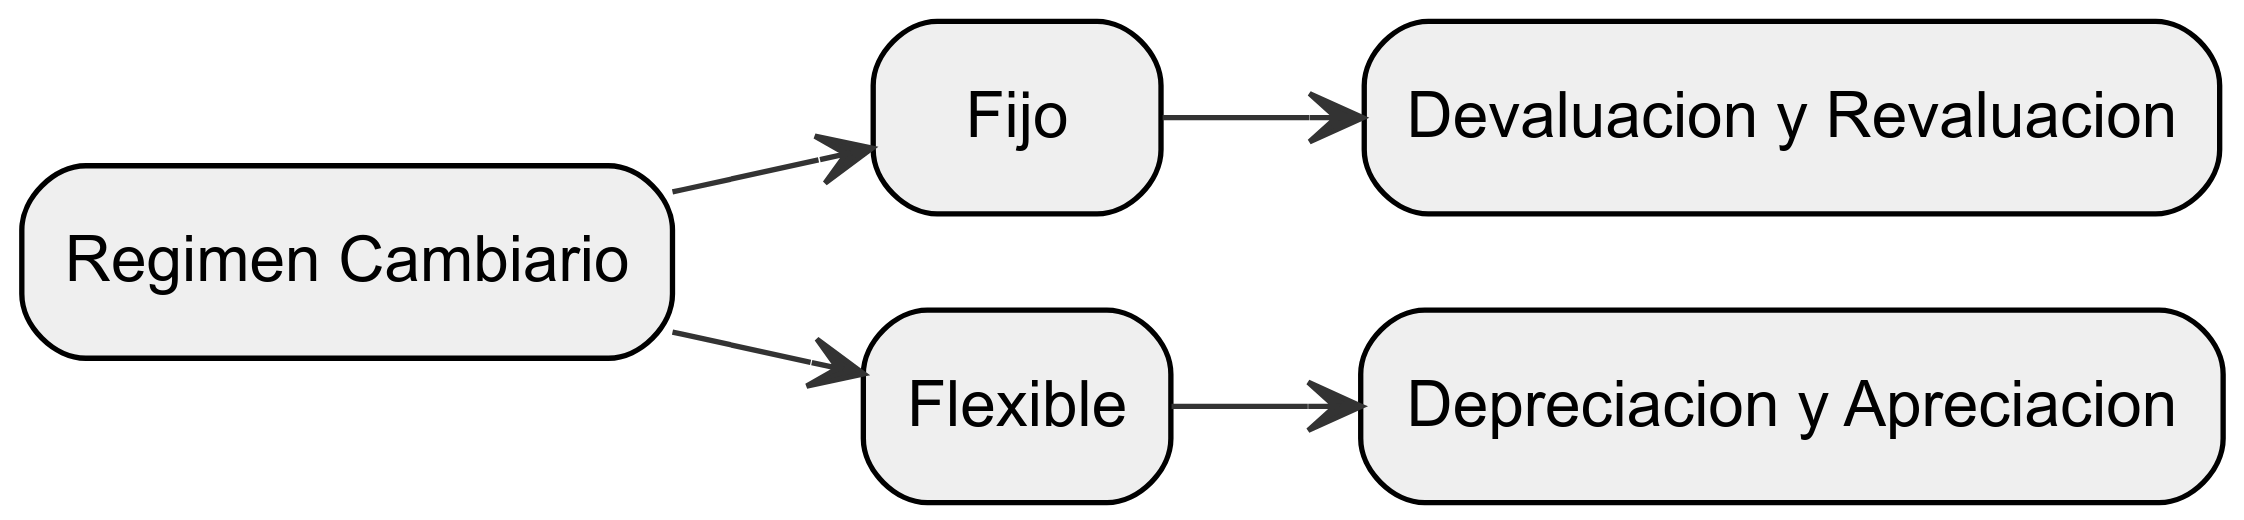
\includegraphics[width=5.5in,height=3.5in]{index_files/figure-latex/dot-figure-1.png}

}

\end{figure}

}

\end{figure}

En una economía abierta, la política cambiaria juega un papel crucial en
la consecución de los objetivos de la política macroeconómica, que
incluyen el logro de un equilibrio tanto interno como externo.

Dado que las economías abiertas se enfrentan a diversos desafíos, la
conducción de la política cambiaria depende de las prioridades
establecidas en variables clave como la inflación, el desempleo, las
tasas de interés, la balanza comercial y el crecimiento económico. Estas
variables influyen en la toma de decisiones relacionadas con el tipo de
cambio y su gestión.

La evolución del sistema monetario internacional en el siglo XX ha
estado marcada por la confrontación entre regímenes cambiarios fijos y
flexibles, así como por la búsqueda de un equilibrio tanto interno como
externo en los objetivos macroeconómicos. Esta historia refleja los
esfuerzos constantes por encontrar el enfoque más adecuado para manejar
las fluctuaciones cambiarias y mantener la estabilidad en la economía
global.

Es importante tener en cuenta que ningún régimen cambiario puede
funcionar eficientemente si no se complementa con políticas fiscales y
monetarias responsables y prudentes. Estas políticas son fundamentales
para respaldar y fortalecer el régimen cambiario elegido, garantizando
así su efectividad y sostenibilidad a largo plazo.

\begin{figure}

\caption{\label{fig-2}Interrelaciones entre tipo de cambio, variables y
políticas económicas}

{\centering 

\begin{figure}[H]

{\centering 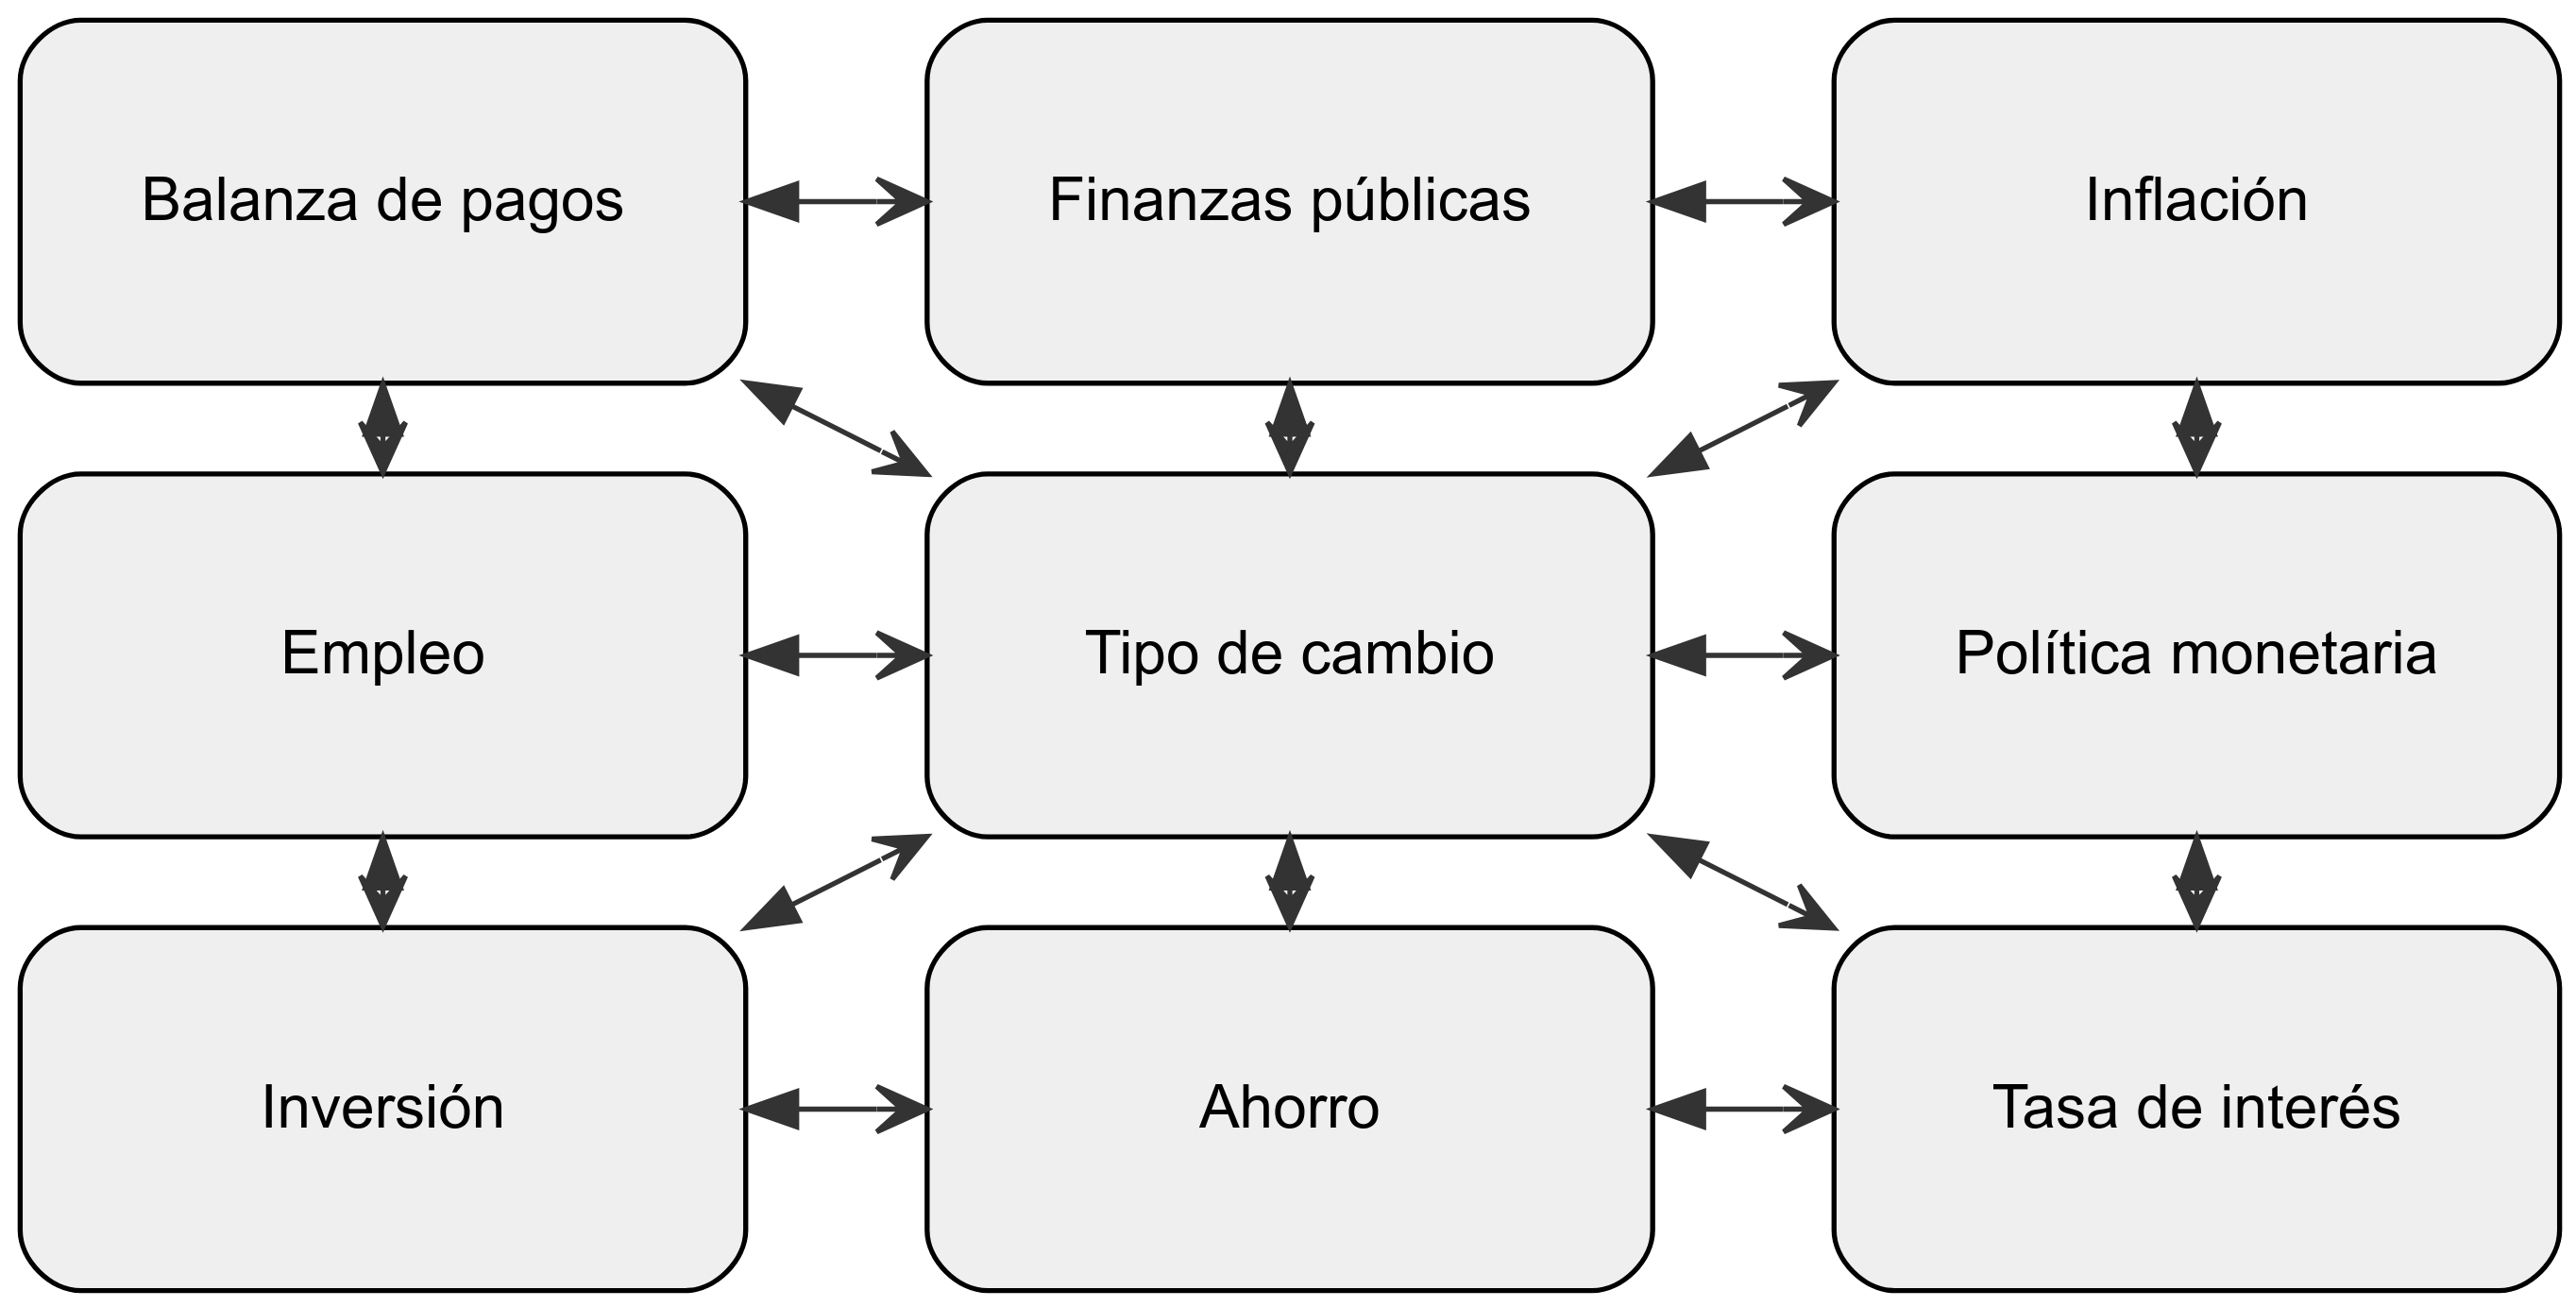
\includegraphics[width=5.5in,height=3.5in]{index_files/figure-latex/dot-figure-2.png}

}

\end{figure}

}

\end{figure}

\hypertarget{la-uniuxf3n-monetaria-europea-y-el-euro}{%
\section{La Unión Monetaria Europea y el
Euro}\label{la-uniuxf3n-monetaria-europea-y-el-euro}}

En 1979, los países de la Comunidad Económica Europea (CEE)
establecieron el Sistema Monetario Europeo (SME) con el objetivo de
crear una zona de estabilidad monetaria en Europa, coordinar políticas
cambiarias y preparar el camino para la Unión Económica Europea. Sin
embargo, el sistema no logró su funcionamiento óptimo debido a la falta
de coordinación de las políticas macroeconómicas entre los países
miembros.

\hypertarget{la-creaciuxf3n-del-euro-y-la-uniuxf3n-monetaria-europea}{%
\subsection{La creación del Euro y la Unión Monetaria
Europea}\label{la-creaciuxf3n-del-euro-y-la-uniuxf3n-monetaria-europea}}

En 1991, los 12 miembros de la CEE firmaron el Tratado de Maastricht, el
cual estableció un cronograma para la creación de la Unión Europea (UE)
con una moneda común, el Euro, y un banco central común. Los países
acordaron coordinar sus políticas fiscales y monetarias, y se
establecieron criterios de convergencia.

\hypertarget{los-compromisos-y-criterios-de-convergencia}{%
\subsection{Los compromisos y criterios de
convergencia}\label{los-compromisos-y-criterios-de-convergencia}}

Cada país se comprometió a mantener el déficit presupuestario por debajo
del 3\% del Producto Interno Bruto (PIB), la deuda pública por debajo
del 60\% del PIB, lograr una baja inflación y mantener el tipo de cambio
dentro de un rango establecido.

\hypertarget{ventajas-del-euro-y-la-uniuxf3n-monetaria}{%
\subsection{Ventajas del Euro y la Unión
Monetaria}\label{ventajas-del-euro-y-la-uniuxf3n-monetaria}}

La adopción del Euro ha generado diversas ventajas para los países
miembros de la UE, entre las cuales se destacan:

\begin{enumerate}
\def\labelenumi{\arabic{enumi}.}
\item
  \textbf{Reducción de los costos de transacción:} Estimaciones indican
  que los costos de transacción se redujeron en un 0.4\% del PIB en la
  UE.
\item
  \textbf{Eliminación de la incertidumbre cambiaria:} El Euro ha
  fomentado la competencia y la inversión al eliminar la volatilidad en
  los tipos de cambio.
\item
  \textbf{Homogeneización y reducción de precios:} El Euro ha
  contribuido a la homogeneización y reducción de precios en la zona
  Euro.
\item
  \textbf{Promoción del comercio y la reestructuración industrial:} La
  moneda común ha impulsado el comercio y la reestructuración industrial
  a nivel continental, lo que ha aumentado la eficiencia y
  competitividad de la economía europea.
\item
  \textbf{Desarrollo de un mercado de capital:} La Unión Monetaria ha
  fomentado el desarrollo de un mercado de capital en la zona Euro,
  reduciendo los costos de capital para las empresas y brindando
  oportunidades a los inversionistas.
\item
  \textbf{Cooperación política y paz:} El Euro ha contribuido a una
  mayor cooperación política entre los países miembros y se considera un
  factor de estabilidad que promueve la paz en Europa.
\end{enumerate}

\hypertarget{desventajas-de-la-moneda-comuxfan}{%
\subsection{Desventajas de la moneda
común}\label{desventajas-de-la-moneda-comuxfan}}

A pesar de las ventajas mencionadas, la moneda común también presenta
ciertas desventajas:

\begin{enumerate}
\def\labelenumi{\arabic{enumi}.}
\item
  Pérdida de soberanía monetaria y cambiaria: Los gobiernos de los
  países miembros pierden la capacidad de tomar decisiones
  independientes en materia monetaria y cambiaria.
\item
  Choques asimétricos y recursos limitados: En caso de enfrentar un
  choque asimétrico, el único recurso para un país afectado es la
  deflación y la reducción de salarios nominales, lo que puede generar
  dificultades económicas y sociales.
\item
  Impacto diferencial en países con monedas fuertes y débiles: Al
  adoptar el Euro, los países que tenían monedas débiles, como Italia y
  España, han experimentado beneficios relativos en comparación con
  países que tenían monedas fuertes, como Alemania y los Países Bajos.
\end{enumerate}

\hypertarget{historia-del-sistema-monetario-internacional}{%
\section{Historia del sistema monetario
internacional}\label{historia-del-sistema-monetario-internacional}}

\hypertarget{el-patruxf3n-oro-cluxe1sico-1875-1914}{%
\subsection{El patrón oro clásico:
1875-1914}\label{el-patruxf3n-oro-cluxe1sico-1875-1914}}

En el periodo del patrón oro clásico, que abarcó desde 1875 hasta 1914,
el sistema monetario internacional se basaba en el uso del oro como
respaldo y base monetaria. Este sistema implicaba que la cantidad de
dinero en circulación en cada país estaba limitada por la cantidad de
oro que poseía. El patrón oro garantizaba la estabilidad del valor del
dinero y establecía mecanismos de ajuste para corregir los
desequilibrios en la balanza de pagos.

\textbf{Ajuste a los desequilibrios en la balanza de pagos bajo el
patrón oro}

Existían dos mecanismos principales para corregir los desequilibrios en
la balanza de pagos bajo el patrón oro. El primero, propuesto por los
economistas clásicos, se basaba en la relación entre la balanza de
pagos, la cantidad de dinero en la economía, el nivel de precios y las
tasas de interés. En caso de un déficit en la balanza de pagos, se
producía una salida de oro y una reducción de la oferta monetaria. Esto
a su vez generaba una disminución de los precios internos, mejoraba la
competitividad del país en términos de exportaciones y reducía las
importaciones. Además, las tasas de interés se incrementaban, lo que
atraía capital extranjero en el corto plazo. Estos ajustes permitían
restablecer el equilibrio externo.

El enfoque mercantilista, que proponía restricciones al comercio para
evitar la salida de oro, fue refutado por Hume. Él demostró que la
riqueza de un país no dependía de la acumulación de oro, sino de su
capacidad de producción de bienes y servicios. El proceso de ajuste bajo
el patrón oro era automático y rápido, pero requería una disminución de
la actividad económica (recesión) para lograr una reducción de los
precios (deflación), lo que afectaba el nivel de vida de la población.

\textbf{Reglas del juego y costos sociales}

Para facilitar el ajuste bajo el patrón oro, se establecieron reglas del
juego. En caso de un déficit en la balanza de pagos, el banco central
del país estaba obligado a vender activos internos (instrumentos de
deuda) para reducir aún más la base monetaria y acelerar el ajuste. Esto
incrementaba las tasas de interés y restringía el crédito. Respetar
estas reglas hacía el proceso de ajuste más doloroso pero más rápido.

Sin embargo, los países superavitarios no siempre respetaban estas
reglas, lo que recaía principalmente en los países deficitarios. Esto
generaba inestabilidad interna y resultaba en recesiones frecuentes y
profundas. Aunque el patrón oro se caracterizó por una baja inflación,
los costos sociales de este sistema fueron elevados.

\textbf{Limitaciones y práctica del ajuste bajo el patrón oro}

En la práctica, el mecanismo de ajuste no siempre funcionaba como se
describía en la teoría. La reducción de los precios era poco frecuente
debido a las políticas de esterilización implementadas por las
autoridades monetarias y a la rigidez de los precios a la baja. Se
requería un largo periodo de recesión para que los precios disminuyeran.
En realidad, el incremento de las importaciones, principal causante de
los desequilibrios en la balanza de pagos, resultaba en una reducción de
la actividad económica debido al desplazamiento de la demanda interna,
la disminución de la inversión y la reducción de los ingresos de la
población.

Investigaciones empíricas del periodo del patrón oro revelan que el
mecanismo real de ajuste se basaba en los movimientos de capital a corto
plazo, atraídos por las altas tasas de interés. Además, se producía una
reducción de la actividad económica en los países deficitarios. Los
precios solo bajaban en raras ocasiones. Ante este escenario, las
autoridades buscaban alternativas no recesivas para lograr el equilibrio
externo, como el proteccionismo, restricciones a los movimientos
internacionales de capital y políticas de esterilización.

\hypertarget{el-periodo-de-entreguerras-1918-1939}{%
\subsection{El periodo de Entreguerras
(1918-1939)}\label{el-periodo-de-entreguerras-1918-1939}}

El periodo de Entreguerras, que abarca desde 1918 hasta 1939, se
caracterizó por desafíos significativos para el sistema monetario
internacional, especialmente el patrón oro, debido a los efectos de la
Primera Guerra Mundial y la posterior Gran Depresión.

\textbf{El impacto de la Primera Guerra Mundial en el patrón oro}

La Primera Guerra Mundial tuvo un efecto disruptivo en el funcionamiento
del patrón oro. El flujo internacional de bienes y capitales se vio
interrumpido y el oro se convirtió en la única forma de pago externo.
Durante el periodo de 1918 a 1923, Alemania y otros países
experimentaron episodios de hiperinflación sin precedentes en la
historia. Los intentos de regresar al patrón oro, realizados por Estados
Unidos en 1918, Gran Bretaña en 1925 y Francia en 1928, fracasaron
repetidamente.

\textbf{El desafío de establecer tipos de cambio realistas}

El problema no resuelto durante este periodo fue cómo establecer tipos
de cambio que reflejaran las realidades económicas de la posguerra. Los
países que intentaban volver al patrón oro no sabían qué paridad
garantizaría el equilibrio externo. En este sentido, la teoría de la
paridad del poder adquisitivo desempeñó un papel relevante al intentar
determinar las relaciones de cambio que reflejaran el poder adquisitivo
de las diferentes monedas.

\textbf{La Gran Depresión y el abandono del patrón} \textbf{oro}

El periodo de 1929 a 1939 es conocido como la Gran Depresión, y marcó un
hito importante en la historia económica mundial. Con el colapso del
sistema bancario en Austria en 1931, las principales naciones
abandonaron el patrón oro. En 1934, Estados Unidos implementó un patrón
oro modificado, fijando el valor de una onza de oro en 35 dólares. Sin
embargo, todos los intentos de regresar al patrón oro resultaron en
recesiones e inestabilidad política.

\textbf{Devaluaciones competitivas y políticas proteccionistas}

En un intento por resolver los desequilibrios internos, muchos países
recurrieron a devaluaciones competitivas para fomentar su empleo interno
y ``exportar el desempleo'' a otros países. Estas devaluaciones buscaban
aumentar las exportaciones y reducir las importaciones. Además, se
implementaron políticas proteccionistas, como altos aranceles, cuotas y
medidas administrativas, que buscaban ``empobrecer al vecino''. Sin
embargo, estas políticas provocaron represalias y desencadenaron
``guerras comerciales'', perjudicando a todos los participantes.

\textbf{La libre flotación de las principales divisas y la especulación}

Durante la Gran Depresión, la libre flotación de las principales divisas
en los mercados cambiarios no lograba establecer paridades de
equilibrio. Los especuladores sistemáticamente elevaban el valor de las
monedas fuertes y reducían el valor de las monedas débiles, generando
mayores inestabilidades en los tipos de cambio.

\hypertarget{el-sistema-de-bretton-woods-1944-1971-cooperaciuxf3n-monetaria-y-colapso}{%
\subsection{El sistema de Bretton Woods (1944-1971): Cooperación
monetaria y
colapso}\label{el-sistema-de-bretton-woods-1944-1971-cooperaciuxf3n-monetaria-y-colapso}}

El sistema de Bretton Woods, establecido en la Conferencia de Bretton
Woods en julio de 1944, fue un marco internacional diseñado para
promover el crecimiento económico, el comercio y la estabilidad
económica.

\textbf{Los objetivos y requisitos del sistema de Bretton Woods}

El sistema de Bretton Woods se estableció con los siguientes objetivos:

\begin{itemize}
\tightlist
\item
  Promover la cooperación monetaria internacional.
\item
  Facilitar el crecimiento del comercio.
\item
  Mantener la estabilidad de los tipos de cambio.
\item
  Establecer un sistema multilateral de pagos.
\item
  Crear una base de reserva internacional.
\end{itemize}

\textbf{Las instituciones del sistema de Bretton Woods}

El sistema de Bretton Woods se basaba en tres instituciones principales:

\begin{itemize}
\tightlist
\item
  \textbf{Fondo Monetario Internacional (FMI):} Encargado de supervisar
  la cooperación monetaria internacional, proporcionar asistencia
  financiera y promover la estabilidad cambiaria.
\item
  \textbf{Banco Mundial:} Establecido para financiar proyectos de
  desarrollo económico y reducir la pobreza en los países miembros.
\item
  \textbf{Acuerdo General sobre Aranceles Aduaneros y Comercio (GATT):}
  Un acuerdo multilateral destinado a promover el comercio internacional
  y reducir las barreras comerciales.
\end{itemize}

\textbf{El régimen cambiario y el patrón oro de cambio}

El sistema de Bretton Woods se basó en el patrón oro de cambio, donde
cada país fijaba el valor de su moneda en términos de oro o dólares
estadounidenses. Los tipos de cambio debían mantenerse dentro de un
rango de variación del 1\% de su paridad en oro. Para hacer frente a los
desequilibrios temporales, los países utilizaban sus reservas y
préstamos del FMI. En casos de desequilibrios fundamentales, el FMI
permitía ajustes en las paridades.

\textbf{Funcionamiento y evolución del sistema de Bretton Woods}

Durante los primeros años, el sistema de Bretton Woods fue exitoso. Sin
embargo, se enfrentó a desafíos, como la resistencia de los países
industrializados en desequilibrio fundamental para ajustar el valor de
sus monedas y las frecuentes devaluaciones en los países en desarrollo.
Para abordar estos problemas, el FMI realizó ajustes y modificaciones a
su funcionamiento. Además, en 1969 se crearon los Derechos Especiales de
Giro (DEG) como una unidad alternativa de reserva para abordar la
escasez de oro.

\textbf{El problema de la balanza de pagos de Estados Unidos}

Después de la Segunda Guerra Mundial, Estados Unidos experimentó
crecientes déficits en su balanza de pagos. A pesar de ser la moneda de
reserva internacional, la demanda del dólar superó su disponibilidad en
el mercado. Estados Unidos perdió una cantidad significativa de sus
reservas en oro durante este periodo.

\textbf{El colapso del sistema de Bretton Woods}

La incapacidad de Estados Unidos para reducir sus déficits y la falta de
confianza en el dólar condujeron al colapso del sistema. En 1971, se
produjo una fuga masiva de capitales de Estados Unidos debido a las
expectativas de devaluación del dólar. Ante los intentos de algunos
bancos centrales europeos de convertir sus reservas de dólares en oro,
Estados Unidos suspendió la convertibilidad del dólar en oro y
estableció una sobretasa del 10\% a las importaciones. A pesar del
intento del Acuerdo Smithsoniano en 1971 de devaluar el dólar y revaluar
otras monedas, no pudo restablecer la confianza. Finalmente, en 1973,
los principales países adoptaron el régimen cambiario de libre
flotación.

\textbf{Causas del derrumbe del sistema de Bretton Woods}

El sistema de patrón oro de cambio dependía de la confianza
internacional en un solo país, lo cual fue una debilidad estructural.
Los costos de ajuste de los tipos de cambio entre las principales
monedas resultaron elevados en la práctica. Además, las políticas
expansivas de Estados Unidos crearon un fenómeno de ``exportación de la
inflación'', lo que llevó a la libre flotación de las monedas como
opción para evitar ``importar la inflación'' de Estados Unidos.

\hypertarget{el-sistema-monetario-internacional-actual-adaptaciuxf3n-a-las-condiciones-cambiantes-de-la-economuxeda-mundial}{%
\subsection{El sistema monetario internacional actual: Adaptación a las
condiciones cambiantes de la economía
mundial}\label{el-sistema-monetario-internacional-actual-adaptaciuxf3n-a-las-condiciones-cambiantes-de-la-economuxeda-mundial}}

El sistema monetario internacional se encuentra en constante ajuste para
responder a las dinámicas de la economía global. En las últimas dos
décadas, se ha observado una aceleración significativa en el ritmo de
los cambios. En un contexto de profundos cambios estructurales a nivel
mundial, los sistemas de tipos de cambio fijos resultarían inadecuados
para acomodar transformaciones tan dramáticas. Parece ser que, en este
escenario, la opción más viable es el sistema de tipos de cambio
flexibles.

\textbf{Transformación del poder económico y su impacto en el sistema
monetario}

El poder económico relativo de los países y continentes experimenta
constantes cambios. El peso económico de Estados Unidos en la economía
global ha disminuido, pero esto no se debe a una supuesta decadencia del
país, sino al impresionante ascenso económico de naciones asiáticas como
Japón, los ``cuatro tigres'' y, más recientemente, China e India.

\textbf{Desafíos y desequilibrios en el mercado}

El cambio en el poder económico conlleva la aparición de desequilibrios
crecientes en el mercado. El enorme déficit comercial de Estados Unidos
lo convierte en una ``locomotora'' de la economía mundial, y una
recesión grave en ese país podría tener efectos incalculables para las
naciones exportadoras. Además, los precios relativos de productos como
el petróleo, metales, café y semiconductores se modifican
constantemente, y un deterioro brusco en los términos de intercambio
puede llevar a un país superavitario a un déficit comercial.

\textbf{Formación de bloques económicos regionales y la integración de
países comunistas}

En el escenario actual, se están creando bloques económicos regionales
en Europa, América del Norte y Asia. Además, los países que alguna vez
formaron parte del bloque comunista se están integrando a la economía
global, generando nuevos flujos económicos y comerciales.

\textbf{El papel del Fondo Monetario Internacional y los atributos de un
sistema monetario ideal}

Tras el colapso definitivo del sistema de Bretton Woods en 1973, el
Fondo Monetario Internacional (FMI) se vio en la necesidad de buscar un
nuevo rol que justificara su existencia. En este contexto, el FMI ha
asumido diversas funciones para promover la estabilidad económica a
nivel mundial y coordinar esfuerzos internacionales con el objetivo de
perfeccionar el sistema monetario.

El FMI desempeña las siguientes funciones:

\begin{itemize}
\item
  Monitoreo de la política económica de los países miembros para
  identificar fortalezas y debilidades.
\item
  Promoción de políticas fiscales y monetarias responsables que
  contribuyan a la estabilidad económica.
\item
  Impulso al desarrollo del sector privado y los mercados libres,
  facilitando un entorno institucional y político propicio para el
  crecimiento del sector privado.
\item
  Señalización de puntos débiles en las economías nacionales y exigencia
  de medidas correctivas para abordar los desequilibrios económicos.
\item
  Organización de paquetes de rescate para países en dificultades
  financieras.
\item
  Promoción de reformas en los sistemas financieros de los países
  miembros.
\item
  Coordinación de esfuerzos internacionales para mejorar el sistema
  monetario internacional.
\end{itemize}

\textbf{Los atributos de un sistema monetario ideal}

Según algunos teóricos, un sistema monetario ideal debería contar con
los siguientes atributos:

\begin{itemize}
\item
  Tipos de cambio fijos: Establecer tasas de cambio fijas entre las
  distintas monedas para brindar estabilidad en las transacciones
  internacionales.
\item
  Libertad de movimientos internacionales de capital: Permitir la libre
  movilidad de los flujos de capital entre países para fomentar la
  inversión y el desarrollo económico.
\item
  Independencia de las políticas monetarias: Garantizar que cada país
  pueda tomar decisiones autónomas respecto a su política monetaria,
  incluyendo el control sobre su oferta monetaria y las tasas de
  interés.
\end{itemize}

Sin embargo, se plantea el trilema fundamental de la macroeconomía,
donde un país solo puede elegir dos de los tres atributos mencionados.
No es posible mantener simultáneamente un tipo de cambio fijo, un
mercado de capitales abierto y una autonomía monetaria. La mayoría de
los países opta por permitir el libre movimiento de capitales y mantener
una política monetaria independiente.

\textbf{Homogeneización de las políticas económicas en la era de la
globalización}

En los últimos años, se ha observado una homogeneización de facto de las
políticas económicas de los países que se han integrado al proceso de
globalización. Para ser competitivos en este entorno, los países
implementan diversas medidas, como:

\begin{itemize}
\item
  Eliminación de barreras comerciales para fomentar el comercio
  internacional.
\item
  Otorgamiento de autonomía a los bancos centrales y reducción de la
  inflación para mantener la estabilidad monetaria.
\item
  Sanear las finanzas públicas y modernizar el sistema impositivo para
  fortalecer la capacidad fiscal del Estado.
\item
  Desregulación de las economías y fortalecimiento del sistema de
  economía de mercado para promover la competencia y la eficiencia.
\item
  Privatización de empresas estatales y promoción de la competencia para
  impulsar la productividad y la innovación.
\item
  Estímulo del ahorro y la inversión para fomentar el crecimiento
  económico sostenible.
\item
  Inversión en infraestructura física y desarrollo del capital humano
  para mejorar la productividad y la calidad de vida.
\end{itemize}

\hypertarget{el-futuro-del-fondo-monetario-internacional}{%
\section{El Futuro del Fondo Monetario
Internacional}\label{el-futuro-del-fondo-monetario-internacional}}

En vista de los dramáticos cambios en la economía mundial, se plantea la
necesidad de realizar ajustes en la arquitectura del sistema monetario
internacional, establecido hace más de 60 años. En este sentido, el
Fondo Monetario Internacional (FMI) ha sido objeto de críticas y se han
propuesto diversas medidas para fortalecer su rol y capacidad de
respuesta ante los nuevos desafíos. A continuación, se presentan algunas
propuestas de cambio para el FMI.

\begin{enumerate}
\def\labelenumi{\arabic{enumi}.}
\item
  \textbf{Fortalecimiento de la base de capital del FMI:} Se propone
  aumentar los recursos del FMI, tanto a través del incremento de las
  cuotas asignadas a los países miembros como de la posibilidad de
  obtener recursos en los mercados de capital. Además, se sugiere la
  creación y promoción de los Derechos Especiales de Giro (DEG), que son
  activos de reserva internacionales utilizados por los países miembros
  del FMI. Estas medidas permitirían al FMI contar con los recursos
  necesarios para hacer frente a las crisis económicas globales.
\item
  \textbf{Reajuste de la representación y votación:} Se propone otorgar
  mayor peso y participación en la toma de decisiones del FMI a los
  países de Asia, América Latina y África. Actualmente, la distribución
  de votos en el FMI se basa en el PIB nominal de los países miembros,
  lo cual favorece a los países industrializados. Se sugiere que los
  votos se calculen en función del PIB estimado con base en la paridad
  del poder adquisitivo (PPA), lo que reduciría la proporción de votos
  de los países industrializados y promovería una mayor
  representatividad.
\item
  \textbf{Reestructuración del Directorio Ejecutivo:} Es necesario
  realizar cambios en la composición y representación del Directorio
  Ejecutivo del FMI. Actualmente, Europa tiene una proporción
  desproporcionada de representantes en comparación con Asia. Se propone
  ajustar esta distribución para reflejar de manera más precisa la
  participación de cada región en el PIB mundial, según la PPA. Además,
  se busca mejorar la rendición de cuentas y transparencia en el
  funcionamiento del Directorio Ejecutivo.
\item
  \textbf{Transformación del FMI en un ``Consejo de Seguridad
  Económica'':} Se plantea convertir al FMI en un prestamista universal
  de última instancia, enfocándose en brindar asistencia en situaciones
  de crisis de liquidez a corto plazo, en lugar de proporcionar
  préstamos a largo plazo para reformas estructurales. Bajo este
  concepto, el FMI actuaría como un ``Consejo de Seguridad Económica'' y
  se centraría en garantizar la estabilidad y confianza en el sistema
  financiero internacional.
\end{enumerate}

\hypertarget{comparaciuxf3n-entre-tipos-de-cambio-fijos-y-flexibles-caracteruxedsticas-y-consecuencias}{%
\section{Comparación entre Tipos de Cambio Fijos y Flexibles:
Características y
Consecuencias}\label{comparaciuxf3n-entre-tipos-de-cambio-fijos-y-flexibles-caracteruxedsticas-y-consecuencias}}

En el ámbito del sistema monetario internacional, existen diferentes
enfoques en cuanto a la gestión de los tipos de cambio. Dos de los
enfoques principales son los tipos de cambio fijos y los tipos de cambio
flexibles. A continuación, se analizan las características y las
consecuencias de cada uno de ellos.

\hypertarget{tipos-de-cambio-fijos}{%
\subsection{Tipos de cambio fijos}\label{tipos-de-cambio-fijos}}

Los tipos de cambio fijos se caracterizan por mantener una paridad
establecida entre las monedas de diferentes países. Algunas de las
características y consecuencias asociadas son las siguientes:

\begin{enumerate}
\def\labelenumi{\arabic{enumi}.}
\item
  \textbf{Ajuste automático:} Cuando se producen desequilibrios en la
  balanza de pagos, el ajuste se realiza mediante la modificación de la
  paridad establecida. Esto implica que el proceso de ajuste es
  automático y no requiere intervención activa por parte de las
  autoridades monetarias.
\item
  \textbf{Ajuste gradual y de bajo costo:} Los cambios en los tipos de
  cambio bajo un sistema de tipo fijo suelen ser graduales y de bajo
  costo. Esto permite una mayor estabilidad en los flujos comerciales y
  financieros entre los países.
\item
  \textbf{Confianza en la economía:} La eliminación de las devaluaciones
  catastróficas, que suelen estar asociadas con los tipos de cambio
  flexibles, aumenta la confianza en la economía. Los agentes económicos
  tienen mayor certidumbre en cuanto a los precios y las transacciones
  internacionales.
\item
  \textbf{Reservas internacionales:} En un sistema de tipo de cambio
  fijo, no es necesario mantener grandes reservas internacionales para
  intervenir en el mercado cambiario. Esto puede resultar beneficioso
  para los países, ya que las reservas pueden destinarse a otros fines.
\item
  \textbf{Independencia de las políticas monetarias:} Bajo un tipo de
  cambio fijo, las autoridades monetarias no están sujetas a las
  exigencias del equilibrio externo. Tienen mayor margen de maniobra
  para implementar políticas monetarias orientadas al logro de objetivos
  internos, como el control de la inflación o el fomento del crecimiento
  económico.
\end{enumerate}

\hypertarget{tipos-de-cambio-flexibles}{%
\subsection{Tipos de cambio flexibles}\label{tipos-de-cambio-flexibles}}

Por otro lado, los tipos de cambio flexibles permiten que las tasas de
cambio se determinen libremente en los mercados de divisas. A
continuación, se presentan las características y las consecuencias
asociadas a este enfoque:

\begin{enumerate}
\def\labelenumi{\arabic{enumi}.}
\item
  \textbf{Liberalización de los movimientos de capital:} Con los tipos
  de cambio flexibles, se fomenta la liberalización de los flujos
  internacionales de capital. Esto implica que los inversionistas tienen
  mayor libertad para realizar operaciones financieras en diferentes
  países.
\item
  \textbf{Crecimiento de los mercados financieros internacionales:} Al
  permitir la fluctuación de los tipos de cambio, se promueve el
  crecimiento de los mercados financieros internacionales. Los
  inversores pueden aprovechar las oportunidades de arbitraje y
  diversificación a nivel global.
\item
  \textbf{Reversibilidad de las depreciaciones:} En un sistema de tipo
  de cambio flexible, las depreciaciones de una moneda no necesariamente
  se traducen de inmediato en un incremento de los precios internos.
  Esto puede brindar cierta flexibilidad a las economías en términos de
  ajuste frente a choques externos.
\end{enumerate}


\printbibliography


\end{document}
